
Performance and its variability can be summarized by a variety of statistics. Mean, range, standard deviation, variance, and interquartile range are a few summary statistics that describe performance and variability. However, the most precise characterization of any performance measure is the cumulative distribution function (CDF), or its derivative the probability density function (PDF). Previous techniques for predicting system performance have strictly modeled real-valued summary statistics because there exists a large base of mathematical techniques capable of approximating functions of the form $f: \mathbb{R}^d \rightarrow \mathbb{R}$. However, there is little systems work approximating functions $f: \mathbb{R}^d \rightarrow \{g \mid g: \mathbb{R} \rightarrow \mathbb{R}\}$.

%% ===================================================================
\section{Measuring Error}
\label{sec:error}

\begin{figure}
  \centering
  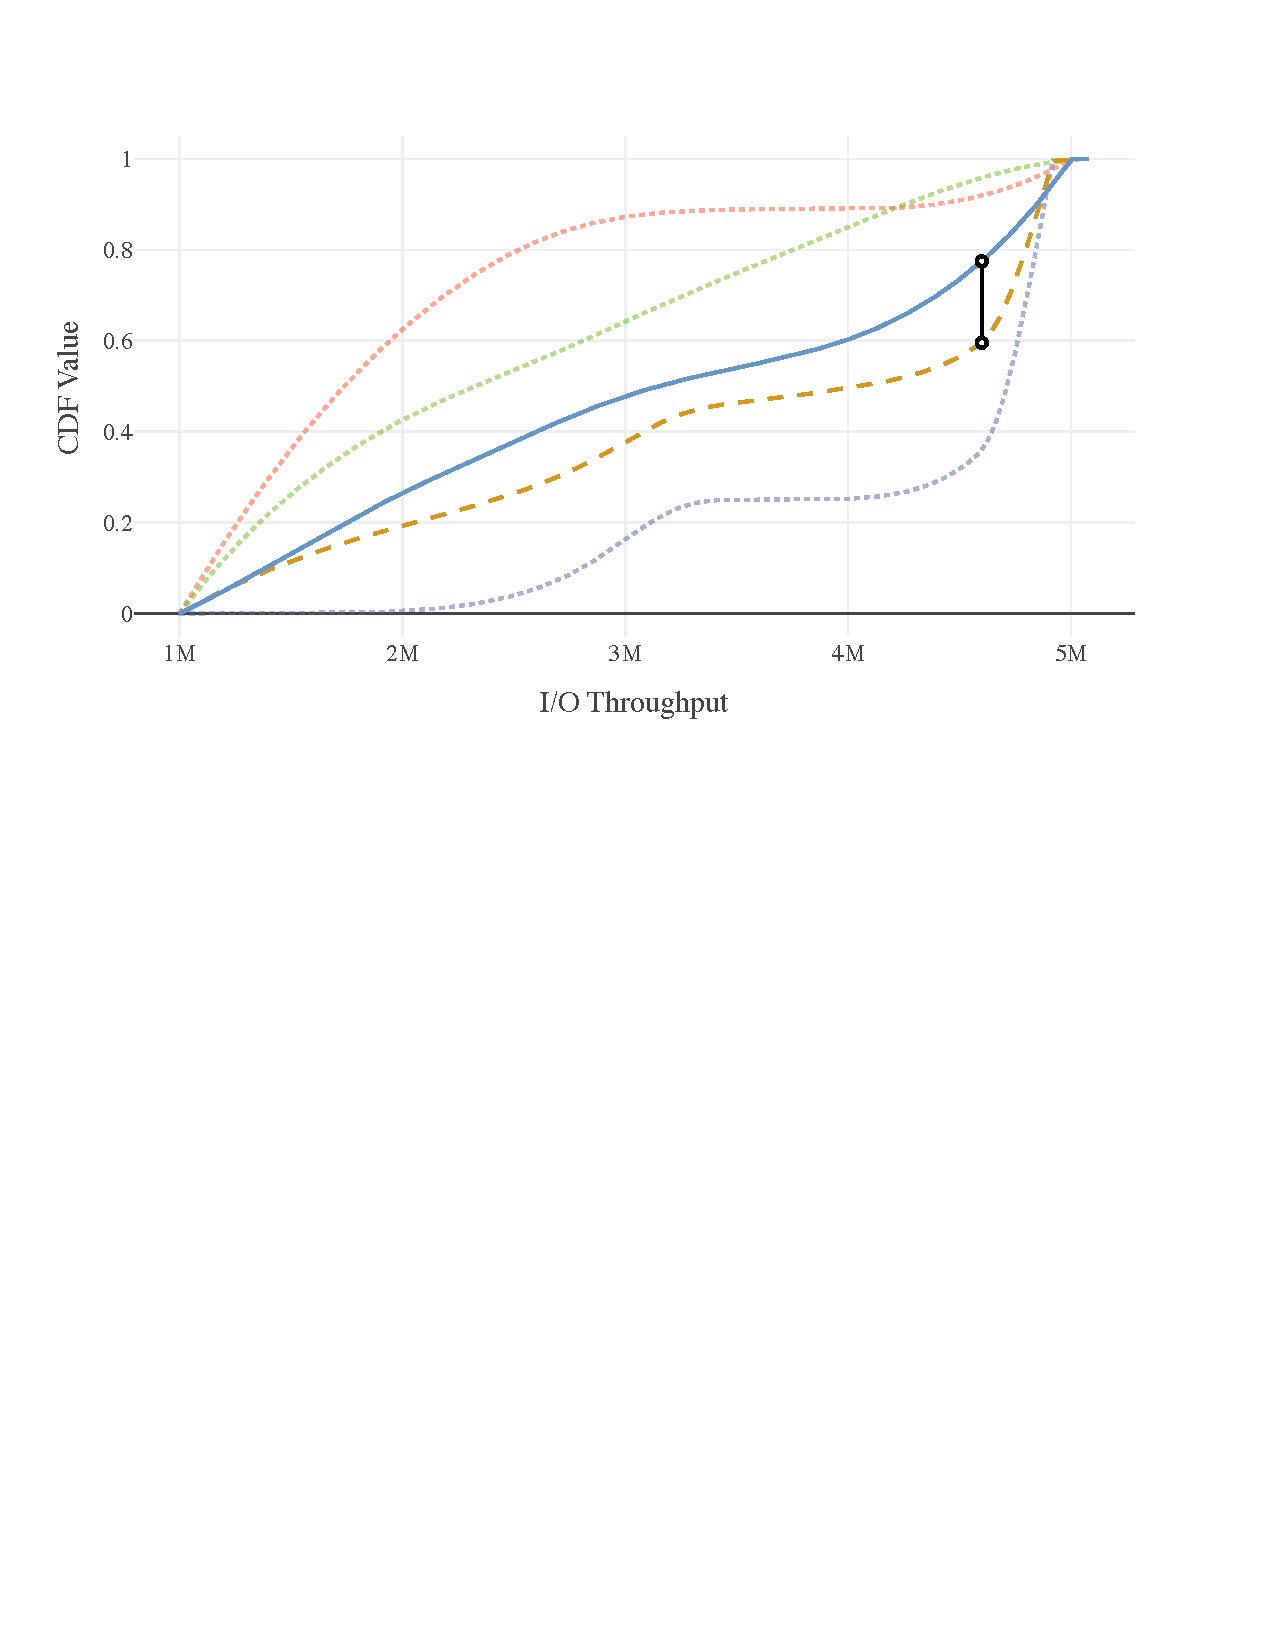
\includegraphics[width=0.8\textwidth,]{Figures/NA/example_distribution_prediction.pdf}
  \caption{In this HPC I/O example, the general methodology for
    predicting a CDF and evaluating error can be seen, where M means
    $\times 10^6$. The Delaunay method chose three source
    distributions (dotted lines) and assigned weights \{.1, .3, .6\}
    (top to bottom at middle). The weighted sum of the three known
    CDFs produces the predicted CDF (dashed line). The KS Statistic
    (vertical line) computed between the true CDF (solid line) and
    predicted CDF (dashed line) is 0.2 for this example. For this
    example the KS test null hypothesis is rejected at $p$-value 0.01,
    however it is not rejected at $p$-value 0.001.
  \vspace{-.1cm}}
  \label{fig:prediction-example}
\end{figure}

When the range of an approximation is the real numbers, error is
reported with summary statistics including: min absolute error, max
absolute error, and absolute error quartiles. When the range
of an approximation is the space of cumulative distribution functions,
the Kolmogorov-Smirnov statistic (max-norm difference between the
functions) is used.

A hurdle when modeling function-valued outputs such as cumulative
distribution functions (CDFs) or probability density functions (PDFs)
is that certain properties must be maintained. It is necessary that a
PDF $f: \mathbb{R} \rightarrow \mathbb{R}$ have the properties $f(x)
\geq 0$ and $\int_{-\infty}^{\infty}f(x)dx = 1$. Instead, for a CDF
$F: \mathbb{R} \rightarrow \mathbb{R}$ the properties are
$F(x) \in [0,1]$ and $F(x)$ is absolutely continuous and
nondecreasing. This work utilizes the fact that a convex combination
of CDFs (or PDFs) results in a valid CDF (or PDF). Given $G(x) =
\sum_{i}w_i F_i(x)$, $\sum_{i} w_i = 1$, $w_i \geq 0$, and each $F_i$
is a valid CDF, $G$ must also be a valid CDF. A demonstration of how
this is applied can be seen in Figure \ref{fig:prediction-example}. 
In this example the KS test null hypothesis is rejected at $p$-value
0.01, however it is not rejected at $p$-value 0.001.

The performance of approximation techniques that predict probability
functions can be analyzed through a variety of summary
statistics. This work uses the max absolute difference, also known as
the Kolmogorov-Smirnov (KS) statistic \cite{lilliefors1967kolmogorov}
for its compatibility with the KS test.

The two-sample KS test is a useful nonparametric test for comparing
two empirical CDFs while only assuming stationarity,
finite mean, and finite variance. The null hypothesis (that two
empirical CDFs come from the same underlying distribution)
is rejected at level $p \in [0,1]$ when
 $$ KS > \sqrt{-\frac{1}{2}\ln\biggl(\frac{p}{2}\biggr)}
\sqrt{\frac{1}{n_1} + \frac{1}{n_2}}, $$ with distribution sample
sizes $n_1,n_2 \in \mathcal{N}$. For all applications of the KS test
presented in this work $n_1 = n_2$. An example of the process of
generating predicted distributions from known distributions and the
subsequent calculation of error can be seen in Figure
\ref{fig:prediction-example}. A brief listing of relevant statistical
terms used throughout this work is provided in the Appendix (Section
\ref{sec:appendix}).

%% ===================================================================
\subsection{Feature Weighting}
\label{sec:feature_weighting}

It is well-known that an important procedure in any application of predictive methodologies is identifying those features of the data that are most relevant to making accurate predictions \cite{guyon2003introduction}. Selection strategies such as the floating searches studied in \cite{pudil1994floating} or others compared in \cite{ferri1994comparative} can be too expensive for large approximation problems. Rather, this work poses feature selection as a continuous optimization problem. Let $X$ be an $n \times d$ matrix of $n$ known system configurations with $d$ parameters each normalized to be in $[0,1]$. Define an error function that computes the error of a predictive model trained on $X\hbox{ diag }w$, $w \in \mathbb{R}^d$,  by performing ten random splits with 80\% of the rows of $X\hbox{ diag }w$ for training and 20\% for testing. A minimum of this error function could be considered an optimal weighting of the features of $X$. Minimization is performed using a zero order method in the absence of a readily computable gradient.


%% ===================================================================
\section{Variability Data}
\label{sec:data}

\begin{table}
  \centering
  \begin{tabular}{c|c}
    \hline
    \textbf{System Parameter} & \textbf{Values}\\
    \hline
    File Size (KB) & 4, 16, 64, 256, 1024, 4096, 8192, 16384\\
    \hline
    Record Size (KB) & \multilinecell{4, 8, 16, 32, 64, 128, 256, 512,\\ 1024, 2048, 4096, 8192, 16384}\\
    \hline
    Thread Count & 1, 8, 16, 24, 32, 40, 48, 56, 64\\
    \hline
    Frequency (GHz) & 1.2, 1.6, 2, 2.3, 2.8, 3.2, 3.5\\
    \hline
    Test Type & \multilinecell{Readers, Rereaders, Random Readers, \\ Initial Writers, Rewriters, Random Writers}\\
    \hline
  \end{tabular}
  \caption{A description of system parameters considered for IOzone. Record size must be $\leq$ file size during execution.}
  \label{tab:data_description}
\end{table}

\begin{figure}
  \centering
  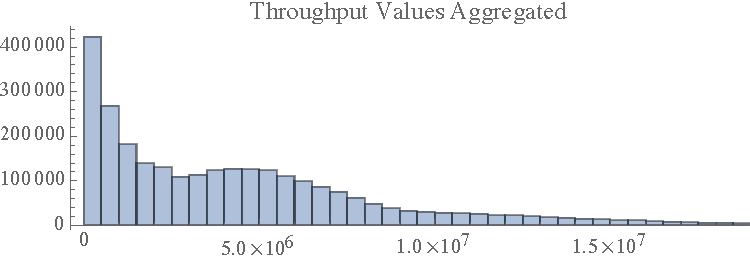
\includegraphics[width=.8\textwidth]{Figures/IEEE/plot-histogram-throughput.pdf}
  \caption{Histogram of the raw throughput values recorded during all IOzone tests across all system configurations. The distribution is skewed right, with few tests having significantly higher throughput than most others.}
  \label{fig:throughput_histogram}
\end{figure}

This chapter utilizes a variability modeling case study with a five-dimensional dataset produced by executing the IOzone benchmark \cite{iozone} on a homogeneous cluster of computers. Each node contains two Intel Xeon E5-2637 CPUs offering a total of 16 CPU cores with 16GB of DRAM. While the CPU frequency varies depending on the test configuration, the I/O from IOzone is performed by an ext4 filesystem sitting above an Intel SSDSC2BA20 SSD drive. At the time of data collection, Linux kernel Version 4.13.0 was used. The system performance data was collected over two weeks by executing IOzone 150 times for each of a select set of approximately 18K system configurations, for a total of approximately 2.7M executions of IOzone. A single IOzone execution reports the max I/O throughput in kilobytes per second seen for the selected test type. The summary of the data components in $x^{(i)}$ for the experiments for this chapter can be seen in Table \ref{tab:data_description}. Distributions of raw throughput values being modeled can be seen in Figure \ref{fig:throughput_histogram}.

Some mild preprocessing was necessary to prepare the data for modeling and analysis. All features were shifted by their minimum value and scaled by their range, mapping each feature independently into $[0,1]$. This normalization ensures each feature is treated equally by the interpolation techniques and should be performed on all data before building models and making predictions regardless of application. All 150 repeated trials for a system configuration were grouped with that configuration. The only nonordinal feature in this data is the test type. All test types were treated as different applications and were separated for modeling and analysis, i.e., predictions for the ``readers'' test type were made using only known configurations for the ``readers'' test type.

%% ===================================================================

\begin{figure}
  \centering
  \begin{tikzpicture}
    \node (img)  {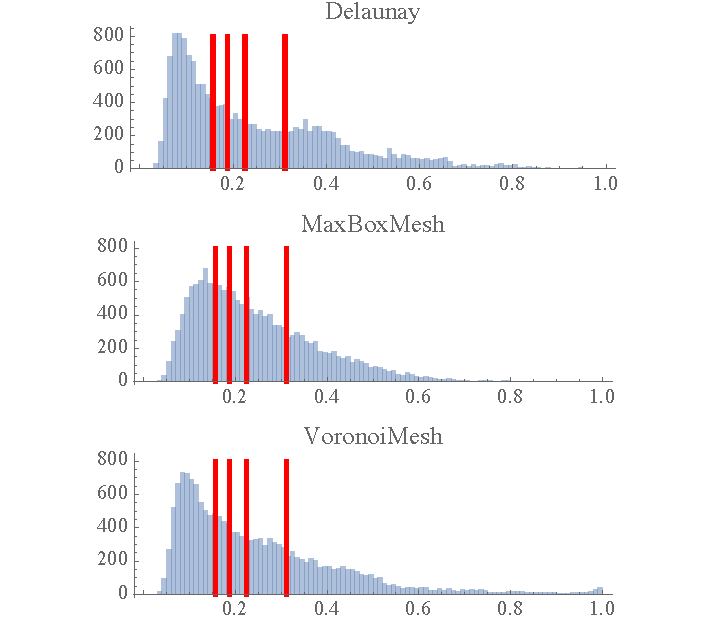
\includegraphics[width=0.8\textwidth,trim={1.5cm 0 0 0}]{Figures/IEEE/plot-histogram-80_20-KS.pdf}};
    \node[below=of img, node distance=1cm, yshift=1cm] {KS Statistic for Predicted vs. Actual};
    \node[left=of img, node distance=0cm, rotate=90, anchor=center,yshift=-0.7cm] {Count of Predictions with Given KS Statistic};
  \end{tikzpicture}
  \caption{Histograms of the prediction error for each modeling algorithm from ten random splits when trained with 80\% of the data aggregated over all different test types. The distributions show the KS statistics for the predicted throughput distribution versus the actual throughput distribution. The four vertical red lines represent commonly used $p$-values \{0.05, 0.01, 0.001, 1.0e-6\} respectively. All predictions to the right of a red line represent CDF predictions that are significantly different (by respective $p$-value) from the actual distribution according to the KS test.}
  \label{fig:ks_histogram_80_20}
\end{figure}

\section{Distribution Prediction Results}

All three interpolation techniques are used to predict the distribution of I/O throughput values at previously unseen system configurations. In order to improve robustness of the error analysis, ten random selections of 80\% of the IOzone data are used to train each model and the remaining 20\% provide approximation error for each model. The recorded errors are grouped by unique system configuration and then averaged within each group. The samples are identical for each interpolation technique, ensuring consistency in the training and testing sets.

The aggregation of errors across all IOzone tests given 80\% of the data as training can be seen in Figure \ref{fig:ks_histogram_80_20}. Agglomerate errors for each technique resemble a Gamma distribution. The percentages of significant prediction errors with varying $p$-values are on display in Table \ref{tab:p_value_failure_rate}. The primary $p$-value used for analyses in this work is 0.001, chosen because close to 2K predictions are made for each test type. Also, applications executed in cloud and HPC systems that could benefit from statistical modeling will be executed at least thousands of times. In line with this knowledge, it is important to ensure that only a small fraction of interpretable results could occur solely under the influence of random chance. When considering the $p=0.001$ results for each technique, a little under half of the predicted CDFs are significantly different from the measured (and presumed) correct CDFs. A rejection rate of 45\% would seem a poor result, however in this situation the complexity of the problem warrants a slightly different interpretation. These predictions are a very \textit{precise} characterization of performance variability, in fact the cumulative distribution function of a random variable is the strongest possible characterization of variability that can be predicted. Globally, only a little under half of the predictions fail to capture \textit{all} of the characteristics of performance variability at new system configurations. It is also demonstrated later in this Section that this result can likely be improved.

\begin{table}
  \centering
  \begin{tabular}{c|c|c}
    \hline
    \textbf{Algorithm} & \textbf{$P$-Value} & \textbf{\% N.H. Rejections} \\
    \hline
    \multilinecell{Delaunay\\Max Box Mesh\\Voronoi Mesh} & .05 & \multilinecell{58.4\\69.3\\61.9}\\
    \hline
    \multilinecell{Delaunay\\Max Box Mesh\\Voronoi Mesh} & .01 & \multilinecell{51.1\\58.4\\53.4}\\
    \hline
    \multilinecell{Delaunay\\Max Box Mesh\\Voronoi Mesh} & .001 & \multilinecell{44.1\\46.9\\45.1}\\
    \hline
    \multilinecell{Delaunay\\Max Box Mesh\\Voronoi Mesh} & 1.0e-6 & \multilinecell{31.4\\26.6\\28.7}\\
    \hline
  \end{tabular}
  \caption{Percent of null hypothesis rejections rate by the KS-test when provided different selections of $p$-values. These accompany the percent of null hypothesis rejection results from Figure \ref{fig:ks_histogram_80_20}.}
  \label{tab:p_value_failure_rate}
\end{table}


While interpreting null hypothesis rejection rates for these interpolation techniques, it is important to consider how the rejection rate reduces with increasing amounts of training data. Figure \ref{fig:ks_failure_by_training} displays the change in $p=0.001$ null hypothesis rejection rate with increasing density of training data up to the maximum density allowed by this set. Delaunay interpolation provides the best results with the least training data by about 5\%, but these low density rejection rates are unacceptably high (90\%). Figure \ref{fig:ks_failure_by_training} clearly shows that this data set and/or the system variables used in the models of performance variability is inadequate to capture the full variability map from system parameters to performance CDF. Which or both obtains is not clear. A few well chosen data points can significantly improve the interpolants, and thus a careful study of the rejection instances is warranted, besides enlarging the set of system variables being modeled.

It may be misleading to consider the global performance of each prediction technique across all test types, as some test types are more difficult than others to predict and have more apparent latent variables. In Figure \ref{fig:ks_failure_by_training_and_test}, the relative difficulty of each IOzone test type can be compared. The I/O test types analyzing reads are typically approximated with lower error than those test types analyzing writes. Regardless of test type, in the aggregate results the KS statistics hover consistently around 0.15, demonstrating an impressively low KS statistic for predictions. In order to address the opacity of aggregate analysis, another case study and an application of the methodology from Section \ref{sec:feature_weighting} is presented in Table \ref{tab:optimized_p_value_failure_rate}.

\begin{figure}
  \centering
  \begin{tikzpicture}
    \node (img)  {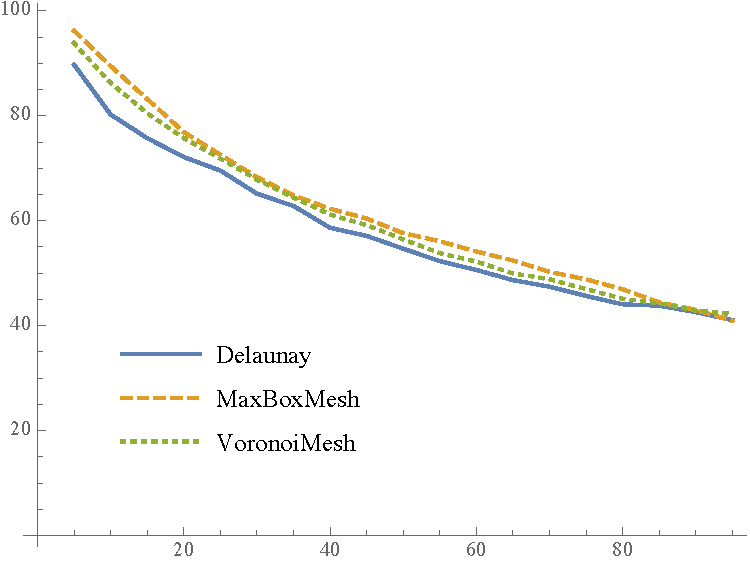
\includegraphics[width=0.8\textwidth,]{Figures/IEEE/plot-KS-Failure-by-Training.pdf}};
    \node[below=of img, node distance=1cm, yshift=1cm] {Percentage of Training Data};
    \node[left=of img, node distance=0cm, rotate=90, anchor=center,yshift=-0.7cm] {\% Null Hypothesis Rejections};
  \end{tikzpicture}
  \caption{The performance of each algorithm on the KS test ($p=0.001$) with increasing amounts of training data averaged over all IOzone test types and ten random splits of the data. The training percentages range from 5\% to 95\% in increments of 5\%. Delaunay is the best performer until 95\% of data is used for training, at which Max Box mesh becomes the best performer by a fraction of a percent.}
  \label{fig:ks_failure_by_training}
\end{figure}

The results presented in Table \ref{tab:optimized_p_value_failure_rate} are achieved by permitting each approximation technique 300 iterations of simulated annealing. In each iteration, the impact of potential weights on the average KS statistic were considered. All weights were kept in the range [0,2], and were applied to the normalized features for frequency, file size, record size, and number of threads. All three approximation techniques had similar optimal weights achieved by simulated annealing of approximately $(.001, 2, 1.7, 1.5)$ for frequency, file size, record size, and number of threads, respectively. Recall that each interpolation technique uses small distances to denote large influences on predictions, meaning that frequency was the most important feature when predicting variability for the ``readers'' test type, followed not-so-closely by number of threads, then record size.

The ``readers'' test type results demonstrate that the underlying prediction techniques work and are capable of seeing rejection rates below 5\% when tuned for a given application. It is important to emphasize that the roughly 95\% of predictions for which the null hypothesis was not rejected are predicting the \textit{precise} distribution of I/O throughput that will be witnessed at a previously unseen system configuration. To the authors' knowledge, there is no existing methodology that is generically applicable to any system performance measure, agnostic of system architecture, and capable of making such powerful predictions.

\begin{table}
  \centering
  \begin{tabular}{c|c|c|c}
    \hline
    \textbf{Algorithm} & \textbf{$P$-Value} & \multilinecell{\textbf{Unweighted}\\\textbf{\% N.H. Rejection}} & \multilinecell{\textbf{Weighted}\\\textbf{\% N.H. Rejection}}\\
    \hline
    \multilinecell{Delaunay\\Max Box Mesh\\Voronoi Mesh} & .05 & \multilinecell{24.9\\21.3\\18.7} & \multilinecell{30.2\\21.2\\11.3}\\
    \hline
    \multilinecell{Delaunay\\Max Box Mesh\\Voronoi Mesh} & .01 & \multilinecell{21.6\\16.4\\14.9} & \multilinecell{27.4\\16.4\\7.0}\\
    \hline
    \multilinecell{Delaunay\\Max Box Mesh\\Voronoi Mesh} & .001 & \multilinecell{19.7\\13.1\\12.3} & \multilinecell{25.4\\13.1\\4.6}\\
    \hline
    \multilinecell{Delaunay\\Max Box Mesh\\Voronoi Mesh} & 1.0e-6 & \multilinecell{17.9\\11.3\\8.5} & \multilinecell{23.4\\11.3\\2.3}\\
    \hline
  \end{tabular}
  \caption{The null hypothesis rejection rates for various $p$-values with the KS-test. These results are strictly for the ``readers'' IOzone test type and show unweighted results as well as the results with weights tuned for minimum error (KS statistic) by 300 iterations of simulated annealing. Notice that the weights identified for the Delaunay model cause data dependent tuning, reducing performance. MaxBoxMesh performance is improved by a negligible amount. VoronoiMesh performance is notably improved.}
  \label{tab:optimized_p_value_failure_rate}
\end{table}

%% \begin{itemize}
%% \item Case studies of good and bad predictions of distributions made, present 3 (best, median, worst)
%% \item Table / Figure showing error for each of the tests (hardest test to predict)
%% \item Presentation of the top most difficult configurations to predict for each test (and the bad performance at those points)
%% %% \item Comparison to predictions made using the "test" numerical column
%% \end{itemize}

\section{Discussion of Distribution Prediction}
\label{sec:discussion}

The results of the IOzone case study indicate that predicting the CDF of I/O throughput at previously unseen system configurations is a challenging problem. The KS statistic captures the worst part of any prediction and hence provides a conservatively large estimate of approximation error. The average absolute errors in the predicted CDFs are always lower than the KS statistics. However, the KS statistic was chosen because of the important statistical theory surrounding it as an error measure. Considering this circumstance, a nonnegligible volume of predictions provide impressively low levels of error. Powerful predictive tools such as those presented in this work allow for more in-depth analysis of system performance variability. For example, system configurations that are most difficult to predict in these tests are likely ``outlier'' configurations that do not resemble those configurations that share many similar parameters. Analysis of these configurations may provide valuable insight into effective application specific operation of computer systems.

As mentioned at the beginning of this chapter, no prior work has attempted to model an arbitrary performance measure for a system to such a high degree of precision. All previous statistical modeling attempts capture a few ($<3$) ordinal performance measures. Generating models that have such high degrees of accuracy allows system engineers to identify previously unused configurations that present desired characteristics. Service level agreements (SLAs) in cloud computing environments are cause for capital competition that is affected heavily by system performance \cite{patel2009service}. Users prefer SLAs that allow the most computing power per monetary unit, incentivizing service providers to guarantee the greatest possible performance. Overscheduling and irregular usage patterns force cloud service providers to occasionally overload machines, in which case precise models of system performance can be used to statistically minimize the probability of SLA violation. Similar targeted performance tuning techniques can be applied to HPC system configuration to maximize application throughput or minimize system power consumption.

A final application domain affected by this methodology is computer security. Collocated users on cloud systems have received attention recently \cite{ali2015security}. If a malicious collocated user is capable of achieving specific insight into the configuration of the system, or the activity of other collocated users by executing performance evaluation programs (i.e., IOzone), a new attack vector may present itself. Malicious users could be capable of identifying common performance distributions of vulnerable system configurations and vulnerable active user jobs. This knowledge may allow targeted exploits to be executed. Light inspection of raw IOzone I/O throughputs provides substantial evidence that distinct performance distributions coincide closely with specific system configuration parameters. Conversely, a service provider may defend against such attacks by deliberately obfuscating the performance of the machine. Models such as those presented in this chapter could identify optimal staggering and time-delay whose introduction into the system would prevent malicious users from identifying system configurations and active jobs.


\begin{figure}
  \centering
  \begin{tikzpicture}
    \node (img)  {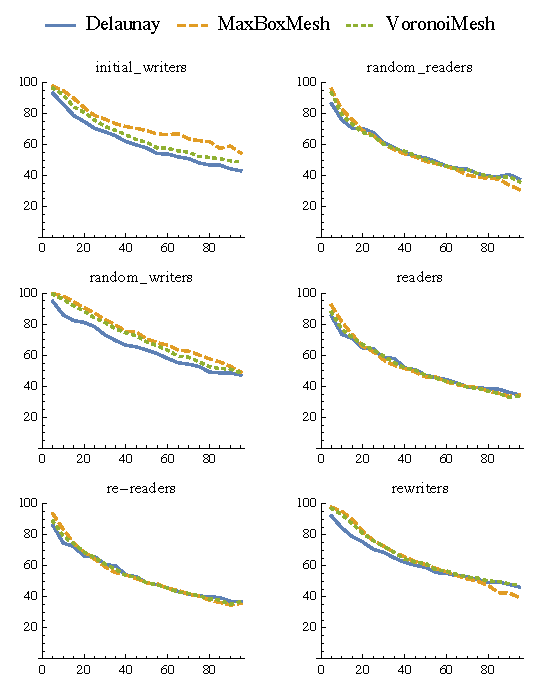
\includegraphics[width=0.8\textwidth,]{Figures/IEEE/plot-KS-failure-by-training-and-test.pdf}};
    \node[below=of img, node distance=1cm, yshift=1cm] {Percentage of Training Data};
    \node[left=of img, node distance=0cm, rotate=90, anchor=center,yshift=-0.7cm] {\% Null Hypothesis Rejections};
  \end{tikzpicture}
  \caption{The percentage of null hypothesis rejections for predictions made by each algorithm on the KS test ($p=0.001$) over different IOzone test types with increasing amounts of training data. Each percentage of null hypothesis rejections is an average over ten random splits of the data. The training percentages range from 5\% to 95\% in increments of 5\%. The read test types tend to allow lower rejection rates than the write test types.}
  \label{fig:ks_failure_by_training_and_test}
\end{figure}


Results presented in Table \ref{tab:optimized_p_value_failure_rate} are particularly interesting, demonstrating that Delaunay appears most vulnerable to data dependent tuning, Max Box mesh is largely insensitive to such tuning, and Voronoi mesh benefits (for this data set) from the tuning.

There are many avenues for extending this modeling methodology. One extension is to add categorical variables to the models. Presently the rejection rate of distribution predictions can only be reduced with large volumes of performance data, however the judicious choice (via experimental design, e.g.) of new data points may be able to effectively reduce the amount of training data required. Finally, more case studies need to be done to test the robustness of the present modeling techniques to changes in domain and performance measure.

\section{The Power of Distribution Prediction}

The methodology presented is capable of providing new insights, extending existing analyses, and improving the management of computational performance variability. Delaunay, Max Box mesh, and Voronoi mesh interpolation are viable techniques for constructing approximations of performance cumulative distribution functions. A case study on I/O throughput demonstrated that the models are capable of effectively predicting CDFs for most unseen system configurations for any of the available I/O test types. The present methodology represents a notable increase in the ability to statistically model arbitrary system performance measures involving the interaction of many ordinal system parameters.
